\documentclass[answers]{exam}
\usepackage[english]{babel}
\usepackage[utf8x]{inputenc}
\usepackage{amsmath,amssymb,amsthm}

\usepackage[table,dvipsnames]{xcolor}
\usepackage{graphicx}
\usepackage{pgf,tikz,tikz-3dplot}
\usetikzlibrary{shapes,arrows,positioning,backgrounds}
\tikzset{%
	roundnode/.style={circle, draw=MidnightBlue!90, thick, fill=gray!40},
	pt/.style={draw=MidnightBlue, thick,->,>=stealth',shorten >=1pt},
	fwd/.style={preaction={draw=YellowOrange,-, line width=2pt,shorten >=3pt}}
}
\usepackage{float}
\usepackage{enumerate}

\begin{document}

\noindent{\large OPER 640 - Stochastic Modeling and Analysis I%
	% Homework X % (Due Jan X at 10am)
	}
\hspace{\fill} {\large B. Hosley}
\bigskip

\begin{questions}

%%%%%%%%%%%%%%%%%%%%%%%%%%%
%	\begin{ Question 1}	  %
%%%%%%%%%%%%%%%%%%%%%%%%%%%
\question 
\emph{Modeling Exercise 2.6 (page 44). Specify both the transition matrix and the transition diagram.}

A machine consists of $K$ components in series,i.e.,all the components must be in working condition for the machine to be functional. When the machine is functional at the beginning of the nth day, each component has a probability $p$ of failing at the beginning of the next day, independent of the other components. (More than one component can fail at the same time.) When the machine fails, a single repair person repairs the failed components one by one. It takes exactly one day to repair one failed component. When all the failed components are repaired the machine is functional again, and behaves as before. When the machine is down, the working components do not fail. Let \(X_n\) be the number of failed components at the beginning of the $n$th day, after all the failure and repair events at that time are accounted for.

Show that \({X_n,n ≥ 0}\) is a DTMC. Display its transition matrix or the transition diagram.
\begin{solution}
	Where the nodes represent the number of broken components:
	
\begin{figure}[H]
	\centering
	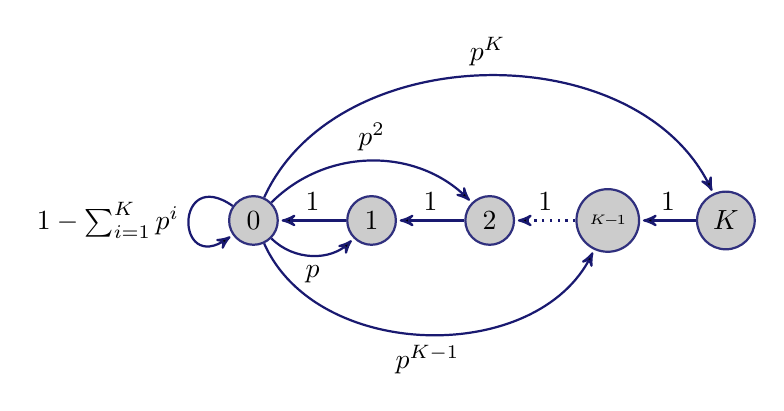
\begin{tikzpicture}[node distance=1.5cm]		
		\node[roundnode] (zero) {0};
		\node[roundnode] (one) [right of=zero] {1};
		\node[roundnode] (two) [right of=one] {2};
		\node[roundnode] (three) [right of=two] {\tiny $K\!\!-\!\!1$};
		\node[roundnode] (four) [right of=three] {$K$};
		
		\path[pt] (one) 	edge []  node [above] 	{1} (zero);
		\path[pt] (two) 	edge []  node [above] 	{1} (one);
		\path[pt] (four) 	edge []  node [above] 	{1} (three);
		\path[pt] (three) 	edge [dotted]  node [above] 	{1} (two);
		
		\path[pt] (zero)	edge [bend right=45]	node [below]	{$p$} (one);
		\path[pt] (zero) 	edge [bend left=45]		node [above]	{$p^2$} (two);
		\path[pt] (zero)	edge [bend right=65]	node [below]	{$p^{K-1}$} (three);
		\path[pt] (zero) 	edge [bend left=65]		node [above]	{$p^K$} (four);
		
		\path[pt] (zero) 	edge [loop left, min distance=9mm, out=145, in=215]	node [left]	{$1-\sum_{i=1}^{K}p^i$} (zero);
	\end{tikzpicture}
	\caption{}
\end{figure}

\begin{align*}
	P =
	\begin{bmatrix}
		1-\sum_{i=1}^{K}p^i & p & p^2 & \cdots & p^{K-1} & p^K \\
		1 & 0 & 0 & \cdots & 0 & 0 \\
		0 & 1 & 0 & \cdots & 0 & 0 \\
		0 & 0 & 1 & \cdots & 0 & 0 \\
		\vdots & \vdots & \vdots & \ddots & \vdots & \vdots \\
		0 & 0 & 0 & \cdots & 0 & 0 \\
		0 & 0 & 0 & \cdots & 1 & 0 \\
	\end{bmatrix}
\end{align*}


\end{solution}
%\end{ Question 1}

%%%%%%%%%%%%%%%%%%%%%%%%%%%
%	\begin{ Question 2}	  %
%%%%%%%%%%%%%%%%%%%%%%%%%%%
\question 
\emph{Modeling Exercise 2.8 (page 45). Specify both the transition matrix and the transition diagram.}

Consider the following weather forecasting model:if today is sunny(rainy)and it is the k-th day of the current sunny (rainy) spell, then it will be sunny (rainy) tomorrow with probability \(p_k (q_k)\) regardless of what happened before the current sunny (rainy) spell started (k ≥ 1). Model this as a DTMC. What is the state-space? What are the transition probabilities?
\begin{solution}
	
	The state space is Sunny (S) and Rainy (R).
	
	\(S=\{\text{S,R}\}\)
	
\begin{figure}[H]
	\centering
	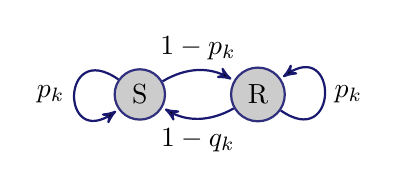
\begin{tikzpicture}[node distance=1.5cm]		
		\node[roundnode] (zero) {S};
		\node[roundnode] (one) [right of=zero] {R};	
		
		\path[pt] (zero)	edge [bend left]	node [above]	{$1-p_k$} (one);
		\path[pt] (one) 	edge [bend left]	node [below]	{$1-q_k$} (zero);
		
		\path[pt] (zero) 	edge [loop left, min distance=9mm, out=145, in=215]	node [left]	{$p_k$} (zero);
		\path[pt] (one) 	edge [loop right, min distance=9mm, out=-35, in=35]	node [right]	{$p_k$} (one);
	\end{tikzpicture}
	\caption{}
\end{figure}

Where Sunny is the $0^{th}$ index and Rainy is $1$.
\begin{align*}
	P =
	\begin{bmatrix}
		p_k & 1-p_k \\
		1-q_k & q_k \\
	\end{bmatrix}
\end{align*}
	
\end{solution}
%\end{ Question 2}

%%%%%%%%%%%%%%%%%%%%%%%%%%%
%	\begin{ Question 3}	  %
%%%%%%%%%%%%%%%%%%%%%%%%%%%
\question 
\emph{Modeling Exercise 2.14 (page 46). Also specify the transition diagram.}

A machine with two components is subject to a series of shocks that occur deterministically one per day. When the machine is working a shock can cause failure of component 1 alone with probability \(\alpha_1\), or of component 2 alone with probability \(\alpha_2\) or of both the components with probability \(\alpha_{12}\) or no failures with probability \(\alpha_0\). (Obviously $\alpha_0+\alpha_1+\alpha_2+\alpha_{12} =1$.)When a failure occurs,the machine is shutdown and no more failures occur until the machine is repaired. The repair time (in days) of component $i (i = 1, 2)$ is a geometric random variable with parameter $r_i , 0 < r_i < 1$. Assume that there is a single repair person and all repair times are independent. If both components fail simultaneously, the repair person repairs component one first, followed by component two. Give the state-space and the transition probability matrix of an appropriate DTMC that can be used to model the state-evolution of the machine.
\begin{solution}
	
	\begin{figure}[H]
		\centering
		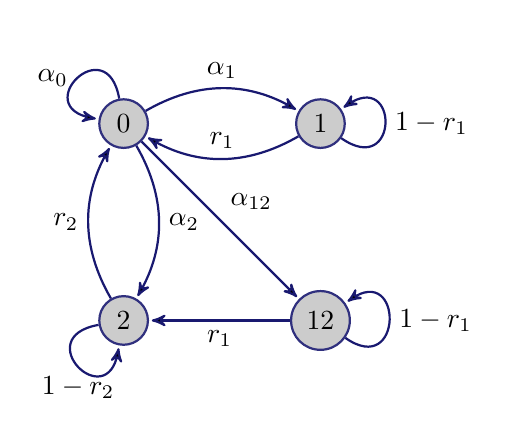
\begin{tikzpicture}[node distance=2.5cm]	
			\node[roundnode] (zero) {0};
			\node[roundnode] (one) [right of=zero] {1};	
			\node[roundnode] (two) [below of=zero] {2};
			\node[roundnode] (three) [right of=two] {12};
				
			\path[pt] (zero) 	edge [loop left, min distance=9mm, out=100, in=170]	node [left]	{$\alpha_0$} (zero);
			\path[pt] (zero)	edge [bend left]	node [above]	{$\alpha_1$} (one);
			\path[pt] (zero)	edge [bend left]	node [right]	{$\alpha_2$} (two);
			\path[pt] (zero)	edge []				node [above right]	{$\alpha_{12}$} (three);
			
			\path[pt] (one) 	edge [loop right, min distance=9mm, out=-35, in=35]	node [right]	{$1-r_1$} (one);
			\path[pt] (one) 	edge [bend left]	node [above]	{$r_1$} (zero);
			
			\path[pt] (two) 	edge [loop right, min distance=9mm, out=-170, in=-100]	node [below]	{$1-r_2$} (two);
			\path[pt] (two) 	edge [bend left]	node [left]	{$r_2$} (zero);
			
			\path[pt] (three) 	edge [loop right, min distance=9mm, out=-35, in=35]	node [right]	{$1-r_1$} (three);
			\path[pt] (three) 	edge []	node [below]	{$r_1$} (two);
			
		\end{tikzpicture}
		\caption{}
	\end{figure}
\end{solution}
%\end{ Question 3}

%%%%%%%%%%%%%%%%%%%%%%%%%%%
%	\begin{ Question 4}	  %
%%%%%%%%%%%%%%%%%%%%%%%%%%%
\question 
Develop a DTMC model of a military-oriented stochastic process. If possible, leverage your own past military experiences.
\begin{solution}
	S
\end{solution}
%\end{ Question 4}

%%%%%%%%%%%%%%%%%%%%%%%%%%%
%	\begin{ Question 5}	  %
%%%%%%%%%%%%%%%%%%%%%%%%%%%
\question 
\textit{Computational Exercise 2.2 (page 51).}

Let \(\{X_n, n \geq 0\}\) be a DTMC with state-space \(\{1, 2, 3, 4, 5\}\) and the following
transition probability matrix:
\[\begin{bmatrix}
	0.1 & 0.0 & 0.2 & 0.3 & 0.4 \\
	0.0 & 0.6 & 0.0 & 0.4 & 0.0 \\
	0.2 & 0.0 & 0.0 & 0.4 & 0.4 \\
	0.0 & 0.4 & 0.0 & 0.5 & 0.1 \\
	0.6 & 0.0 & 0.3 & 0.1 & 0.0 
\end{bmatrix}.\]

Suppose the initial distribution is \(a = [0.5, 0, 0, 0, 0.5]\). Compute the following:
\begin{enumerate}[1.]
	\item The pmf of \(X_2\),
	\item \(P(X_2 = 2, X_4 = 5)\),
	\item \(P(X_7 = 3|X_3 = 4)\),
	\item \(P(X_1 \in \{1,2,3\},X_2 \in \{4,5\})\).
\end{enumerate}
\begin{solution}
	\begin{enumerate}[1.]
		\item \(a^{(2)} = \begin{bmatrix} 0.205 & 0.08 & 0.13 & 0.325 & 0.26 \end{bmatrix}\)
		\item \(aP^{(2)}(2) \times aP^{(4)}(5) = 0.01296\) 
		\item \( \begin{bmatrix} 0 & 0 & 0 & 1 & 0 \end{bmatrix} \times aP^{(7-3)}(3) = 0.0318 \)
		\item \(\sum_{i=1}^{3} a^{(1)}(i) \times \sum_{j=4}^{5} a^{(2)}(j) = 0.351\)
	\end{enumerate}
\end{solution}
%\end{ Question 5}

%%%%%%%%%%%%%%%%%%%%%%%%%%%
%	\begin{ Question 6}	  %
%%%%%%%%%%%%%%%%%%%%%%%%%%%
\question 
\textit{Computational Exercise 2.8 (page 52).}

Let \(\{X_n,n\geq0\}\) be a DTMC with state-space \(\{1,2,3,4\}\) and transition probability matrix given below:
\[P=\begin{bmatrix}
	0.4 & 0.3 & 0.2 & 0.1 \\
	0.5 & 0.0 & 0.0 & 0.5 \\
	0.5 & 0.0 & 0.0 & 0.5 \\ 
	0.1 & 0.2 & 0.3 & 0.4
\end{bmatrix}.\]
Suppose \(X_0 = 1\) with probability 1. Compute:
\begin{enumerate}[1.]
	\item \(P(X_2 = 4)\),
	\item \(P(X_1 = 2, X_2 = 4, X_3 = 1)\), 
	\item \(P(X_7 = 4|X_5 = 2)\),
	\item \(E(X_3)\).
\end{enumerate}
\begin{solution}
	\begin{enumerate}[1.]
		\item \(aP^{(2)}(4)  =  0.33\)
		\item \(aP^{(1)}(2) \times aP^{(2)}(4) \times aP^{(3)}(1)  =  0.032274\)
		\item \(\begin{bmatrix} 0 & 1 & 0 & 0 \end{bmatrix} \times aP^{(7-5)}(4)  =  0.25\)
		\item \(\sum_{i=1}^{4}aP^{(2)}(i) = 2.455\)
	\end{enumerate}
\end{solution}
%\end{ Question 6}

%%%%%%%%%%%%%%%%%%%%%%%%%%%
%	\begin{ Question 7}	  %
%%%%%%%%%%%%%%%%%%%%%%%%%%%
\question 
\textit{Computational Exercise 2.12 (page 52).}

Consider the weather forecasting model of Modeling Exercise 2.5. 
What is the probability distribution of the length of the rainy 
spell predicted by this model? Do the same for the length of the sunny spell.

\begin{solution}
	Let the state space be \{RR, RS, SR, SS\} 
	where the letters correspond to \(n-1,n\) respectively.
	Then the forecasting matrix with indexes corresponding to
	order of the state space above will be:
	\[F= \begin{bmatrix}
		0.6 & 0.4 & 0.0 & 0.0 \\
		0.0 & 0.0 & 0.25 & 0.75 \\
		0.5 & 0.5 & 0.0 & 0.0 \\
		0.0 & 0.0 & 0.2 & 0.8 
	\end{bmatrix}\]
	
	Let \(P_r(l)\) be the probability of a rainy spell consisting of \(l\) days and
	\(P_s(l)\) be the probability of a sunny spell consisting of \(l\) days.
	Then, because a spell always begins when \(n-1\neq n\), the initial states are given:
	\[
	a_r = \begin{bmatrix} 0 & 0 & 1 & 0 \end{bmatrix}, \quad
	a_s = \begin{bmatrix} 0 & 1 & 0 & 0 \end{bmatrix}.
	\]
	And because the last day of a spell is also transitional,
	the index of the end will be the opposite of the start, thus:	
	\begin{align*}
	P_r(l) = a_rF^{(l)}(2) \\
	P_s(l) = a_sF^{(l)}(3).
	\end{align*}
	
	
\end{solution}
%\end{ Question 7}

%%%%%%%%%%%%%%%%%%%%%%%%%%%
%	\begin{ Question 8}	  %
%%%%%%%%%%%%%%%%%%%%%%%%%%%
\question 
Consider a workshop with five identical machines. 
A machine can be either up (i.e., working) or down (i.e., failed). If a machine is up on day n, it will be up on day n + 1 with probability 0.9. If a machine is down on day n and a repair is attempted, it will be up on day n + 1 with probability 0.6. The five machines behave independently of each other. The workshop can attempt to repair no more than two down machines on a single day. Initially, all five machines are down.

\begin{enumerate}[(a)]
	\item Model this system as a DTMC.
	\begin{enumerate}[i.]
		\item Specify the state variable \(X_n\) and the state space S.
		\item Specify the transition probability function \(p_{i,j}\). (Hint: use a convolution of the pmfs of two binomial random variables.)
		\item Specify the transition probability matrix numerically.
		\item Confirm the Markov property and time homogeneity.
	\end{enumerate}
	\item  Compute and display (as separate vertical bar charts) the pmfs of the state variable on days 2, 4, and 8. 
	Label figures appropriately. What do you observe?
	
	\item On one figure, plot the probability the number of up machines is 4 or more and the probability the number of up machines is 1 or fewer for days 0, 1, . . . , 10. Include dashed lines between points. Label the figure appropriately.
	
	\item After seven days of operations (i.e., at the end of Day 6), how many days can the workshop expect to have operated with four or more machines up? What would happen if the workshop began operations with all five machines up?
	
	\item Compute and display the expected value and variance of the system state over time. Plot the expected value of the system state on days 0, 1, . . . , 10 as a solid line with circle markers. Also indicate the standard deviation of the system state (i.e., \(\pm \sqrt{Var(X_n)}\)) by plotting \(\pm 1\)-standard deviation offsets (both higher and lower) from the solid expected value line. These two lines should be dashed.
	
	\item Suppose each machine generates \$1 of revenue per day when it is up. Compute and plot the expected total revenue as of Day 0, 1, . . . , 10.
	(Ensure all figures are appropriately labeled with legends included as required. Ensure the grid of each figure is shown, so detailed information can be discerned.)

\end{enumerate}
\begin{solution}
	\begin{enumerate}[(a)]
		\item 
		\begin{enumerate}[i.]
			\item 
			\item 
			\item 
			\[\begin{bmatrix}
				0.59049 & 0.32805 & 0.0729 & 0.0081 & 0.00045 & 0.00001 \\
				0.39366 & 0.4374  & 0.1458 & 0.0216 & 0.0015  & 0.00004 \\
				0.26244 & 0.4374  & 0.243  & 0.0522 & 0.0048  & 0.00016 \\
				0       & 0.2916  & 0.4536 & 0.2196 & 0.0336  & 0.0016  \\
				0       & 0       & 0.324  & 0.468  & 0.192   & 0.016   \\
				0       & 0       & 0      & 0.36   & 0.48    & 0.16    
			\end{bmatrix}\]
			\item 
		\end{enumerate}
	\end{enumerate}
\end{solution}
%\end{ Question 8}



\end{questions}
\end{document}